%!TEX program = xelatex
% AMOJ requires the use of the XeTeX (xelatex) typesetting engine to produce the correct fonts
% Not using XeTeX is not going to break anything, it just means that your compiled article
% may look a little different to what it's meant to.
% XeTeX comes bundled with most LaTeX distributions, so everything will probably work fine...
\documentclass[10pt]{article}


% Include the amoj package. It's what formats your article correctly
\usepackage{amoj}


% The title should be both brief and descriptive. It must clearly communicate the nature of the article.
% Ideally, your title should incorporate a key phrase related to your topic within the first 65 characters.
\title{Preparing your AMOJ Manuscript}


% Individual author names must be listed in the following style:
% first name then initials with full stops after each initial then last name, followed by any generational suffix.
% Prefixed and post nominal professional titles and academic qualifications should not be included.
%
% Author names should be listed one after the other without line breaks and separated by commas,
% with the exception of the last name of a multi-name list, which should be separated by the word "and" without a comma.
%
% Numbers indicating author affiliations (see above) should be included in supertext after each name or after the separating comma, if one is used.
\author{First A. Author,\textsuperscript{1} Second B. Author\textsuperscript{2} and Third. C. Author\textsuperscript{3}}


% Each affiliation should be as concise as possible and in general should not constitute a complete address,
% rather indicate the primary institution of the author(s) and the city and country that the institution is located in.
%
% Each affiliation should be on its own line.
%
% Affiliations should be preceded by the relevant number in supertext that corresponds with the numbers used in the author line above.
\affiliations{%
\textsuperscript{1} Institution, City, Country\\% These \\%'s are important
\textsuperscript{2} Institution, City, Country\\%
\textsuperscript{3} Institution, City, Country\\%
}

%%%%%%%%%%%%%%%%%%%%%%%%%%%%%%%%
% Provenance Information
% Editorial Office Use Only
%
\msreceived{Month Year}
\msaccepted{Month Year}
\volume{Vol.}
\issue{Issue}
\doi{DOI}
\copyrightyear{2015}
\copyrightauthor{Author et al}
%
%%%%%%%%%%%%%%%%%%%%%%%%%%%%%%%%

\begin{document} % This is important, but you already knew that
\maketitle

%%%%%%%%%%%%%%%%%%%%%%%%%%%%%%%%%%%%%%%%%%%%%%%%%%%%%%%%%%%%%%%%%%%%%%%%%%%%%%%%%%%%%%%%%%%%%%%%%%%%%%%%%%%%%%%%%%%%%%%%%%%%%%%%%%%%%%%%%%%%%%%%%
% Put your abstract here

\begin{abstract}
An abstract is required at the beginning of each article and, at the discretion of the Editor, at the beginning of appropriate shorter contributions. Authors are reminded to summarise their conclusions in the abstract, as well as the methods used, since abstracts are frequently quoted verbatim in abstracting journals.

Authors are encouraged to think about how the words and phrases that a researcher might use to search for their article and include these words and phrases in their abstract in a natural and contextual manner.

Abstracts may consist of multiple paragraphs if absolutely necessary. Headings should not be used in abstracts.
\end{abstract}

%%%%%%%%%%%%%%%%%%%%%%%%%%%%%%%%%%%%%%%%%%%%%%%%%%%%%%%%%%%%%%%%%%%%%%%%%%%%%%%%%%%%%%%%%%%%%%%%%%%%%%%%%%%%%%%%%%%%%%%%%%%%%%%%%%%%%%%%%%%%%%%%%
% Start your article

\section{Introduction (Heading 1 Style)}
For style refer to the publication Style Manual for Authors, Editors and Printers of Australian Government Publications (6th edition, 2002), and to recent issues of the journal.

The main article text (Word style Normal) should be divided into sections, each with a separate heading. Section headings may be up to three levels deep, and must always use the corresponding Word style (Heading 1, Heading 2, and Heading 3). Sections should not be numbered.

\section{Figures}
\label{figures}
Please choose the location where you insert your figure into the template wisely. It should be as close as possible to the location of the first reference in the text, but care must be taken to ensure that the image fits on the page and does not introduce extraneous white space into the article.

Figures can be inserted by clicking on the ``Picture'' button on the ``Insert'' tab of the ribbon. Figures must be centre justified on their own line and have text wrapping should be set to ``In line with text.''

Authors are strongly encouraged to join multi-part figures into a single image before attempting to insert the figure into the article template. 

\subsection{Referencing figures}
\label{referencing_figures}
All figures should be mentioned specifically in the text: e.g. Figure 1.

References to figures in the text should be achieved with the use of cross-references. Guidance on how to use this feature can be found courtesy of the website of the International Electrotechnical Commission.

\begin{figure}
  \centering
    \caption{An example figure.}
    \label{figure:exampleFigure}
    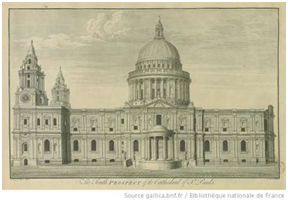
\includegraphics[keepaspectratio=true,width=0.5\textwidth]{example_figure.png}
\end{figure}

\section{Tables}
\label{tables}
Tables can be inserted by clicking on the “Table” button on the “Insert” tab of the Ribbon.

Tables should be styled using the AMOJ Table Style included in the template, accessible via the Table Tools > Design ribbon tab. The AMOJ Table Style is listed in the “Custom” group; the style name can be found by hovering your mouse over the style preview image. 

All tables should be centre justified on the page, and should only be as wide as is necessary to adequately display the content.

Additional horizontal lines may be added to separate groups of cells, if doing so will aid comprehension (see Table 1). These lines must be added manually by changing the “Border” options for the relevant cells. The Microsoft Office support site has an article that explains how to add borders to tables.

Each table must have a brief caption that describes its contents that must be understandable without reference to the text. The captions should be formatted the same as for figures.

\begin{table}[h]
  \centering
    \caption{An example of a table using the AMOJ Table Layout}
    \label{table:exampleTable}
    \begin{AMOJTable}{\textwidth}{XXX}
      \hline \\
      \textit{Column Heading}                                   & \textit{Column Heading}                                                         & \textit{Column Heading}                                                                   \\
      \hline \\
      Lorem ipsum dolor sit amet, consectetur adipisicing elit. & Eius adipisci, sed libero. Iste asperiores suscipit, consequatur debitis animi. & Impedit numquam facilis iusto porro labore dolorem, maxime magni incidunt. Delectus, est! \\
      Lorem ipsum dolor sit amet, consectetur adipisicing elit. & Eius adipisci, sed libero. Iste asperiores suscipit, consequatur debitis animi. & Impedit numquam facilis iusto porro labore dolorem, maxime magni incidunt. Delectus, est! \\
      \hline \\
      Lorem ipsum dolor sit amet, consectetur adipisicing elit. & Eius adipisci, sed libero. Iste asperiores suscipit, consequatur debitis animi. & Impedit numquam facilis iusto porro labore dolorem, maxime magni incidunt. Delectus, est! \\
      Lorem ipsum dolor sit amet, consectetur adipisicing elit. & Eius adipisci, sed libero. Iste asperiores suscipit, consequatur debitis animi. & Impedit numquam facilis iusto porro labore dolorem, maxime magni incidunt. Delectus, est! \\
      \hline
    \end{AMOJTable}
  \end{table}

\section{Figure and table captions}
\label{FigureTableCaptions}
Each figure and table must have an adequate caption set above the figure or table. These captions, and the caption labels, must part of the main article text and not part of the figure or drawing. 

Captions should be added by right clicking on the figure and selecting “Insert caption” or selecting the entire table, right clicking and choosing “Insert caption.” This method will ensure that figures and tables are numbered correctly and that cross-references link to the correct place within the article.

Caption labels (e.g. Figure 1) must be separated from the caption text by a single tab character. Punctuation marks should not be used to separate caption labels and the caption text.

\section{Mathematical symbols and formulae}
\label{MathematicalSymbolsFormualae}
Equations should, where appropriate, be included inline with the main body text. Where this is not possible, equations should be formatted as below. Equations can be easily inserted in the correct format by using the provided AMOJ Equation template. This can be done by clicking the arrow under the equation icon on the Insert tab on the Ribbon and choosing AMOJ Equation from the list of equation templates.

\begin{equation}
e = mc^2
\end{equation}

References in text to equations should be made by the equation number prefixed by Eqn.

The following guidelines should be followed when using equations:
\begin{itemize}
  \item Double-line fractions should not be used in the body of the text. To indicate such fractions, use the solidus (/) or the negative exponent; thus a/b, or ab-1, or b-1a. Double-line fractions should be avoided also in centred equations if they can be expressed conveniently by any of the methods just noted and the resulting equation will appear on only one line.
  \item The radical sign should be avoided. To indicate roots, use a fractional positive or negative exponent.
  \item Avoid double superscripts or subscripts as well as superscripts attached to the same symbol.
  \item Indicate vectors and matrices by placing a wavy line under the symbol. Do not underline any other symbols or use underlining as part of a symbol.
  \item When the number e is modified by a complicated exponent, use the symbol exp.
  \item In writing units, the solidus (/) may be used instead of negative exponents provided ambiguity is avoided: i.e. either J kg-1 K-1 or J/(kg K) is acceptable, but not J/kg/K. Multiple use of the solidus is never justified.
\end{itemize}

\section{Units}
\label{Unites}
The International System of Units is standard in the Southern Hemisphere Earth System Science and SI (m, kg, s, K) units should be used throughout. 

Words and symbols for units should not be mixed; in general, symbols should be used only when preceded by a number (thus `10 m', but `several metres').

Unit symbols are not punctuated, i.e. they are not treated as abbreviations; the same symbol is used for both singular and plural.

Note that, although the Kelvin is the unit of temperature in the SI, the degree sign must be used in writing temperatures or temperature differences in the Celsius scale, i.e. `272 K', but `22 \textdegree C.' 

Day, month and year are written `29 December 1959' (do not abbreviate names of months). 

The recommended time zone is Coordinated Universal Time, abbreviated UTC. Time, time zone, day, month and year are written `2330 UTC 29 December 1959', in some instances the use of other time zones is permissible, for example, AEST (150?E meridian civil time).

\section{Abbreviations}
Unless repetitive, abbreviations should be avoided, especially of organisations (write `World Meteorological Organization' not `WMO'), and acronyms should be identified with their first use, e.g. `clear-air turbulence (CAT).'

\section{Author Contributions}
A section must be included that details the contributions of each author to the preparation of the manuscript and the underlying study.

Immediately following this, the contact details of the corresponding author must appear, including:
\begin{itemize}
  \item Full name;
  \item Email address; and
  \item Full postal address, including country.
\end{itemize}

\section{Acknowledgments}
\label{Acknowledgments}
The last paragraph of the article is the place to acknowledge people, places, and funding. Acknowledgements can contain multiple paragraphs.


%%%%%%%%%%%%%%%%%%%%%%%%%%%%%%%%%%%%%%%%%%%%%%%%%%%%%%%%%%%%%%%%%%%%%%%%%%%%%%%%%%%%%%%%%%%%%%%%%%%%%%%%%%%%%%%%%%%%%%%%%%%%%%%%%%%%%%%%%%%%%%%%%
% Automagically insert a reference list
\bibliography{references-samplecontent}

%%%%%%%%%%%%%%%%%%%%%%%%%%%%%%%%%%%%%%%%%%%%%%%%%%%%%%%%%%%%%%%%%%%%%%%%%%%%%%%%%%%%%%%%%%%%%%%%%%%%%%%%%%%%%%%%%%%%%%%%%%%%%%%%%%%%%%%%%%%%%%%%%

\subsection{Reference list}
\label{ReferenceList}
References should be placed at the very end of the article.

References must follow the Harvard referencing style.

Authors are responsible for the accuracy and completeness of all references.

\subsection{In-text citations}
\label{IntextCitations}
In-text citations citation should consist of the name of the author and the year of publication. Thus, `according to \citet{David2013,Linden2009,Trewin2010}', or `as shown by an earlier study \cite{Budin1985}'. When there are two or more papers by the same author published in the same year, the distinguishing letters a, b, etc., should be added to the year.


\section{Appendix}
\label{Appendix}
Lengthy mathematical analyses whose details are subordinate to the main theme of the paper should normally be put into an appendix.

\end{document}
